\documentclass{article}\usepackage{graphicx, color}
%% maxwidth is the original width if it is less than linewidth
%% otherwise use linewidth (to make sure the graphics do not exceed the margin)
\makeatletter
\def\maxwidth{ %
  \ifdim\Gin@nat@width>\linewidth
    \linewidth
  \else
    \Gin@nat@width
  \fi
}
\makeatother

\IfFileExists{upquote.sty}{\usepackage{upquote}}{}
\definecolor{fgcolor}{rgb}{0.2, 0.2, 0.2}
\newcommand{\hlnumber}[1]{\textcolor[rgb]{0,0,0}{#1}}%
\newcommand{\hlfunctioncall}[1]{\textcolor[rgb]{0.501960784313725,0,0.329411764705882}{\textbf{#1}}}%
\newcommand{\hlstring}[1]{\textcolor[rgb]{0.6,0.6,1}{#1}}%
\newcommand{\hlkeyword}[1]{\textcolor[rgb]{0,0,0}{\textbf{#1}}}%
\newcommand{\hlargument}[1]{\textcolor[rgb]{0.690196078431373,0.250980392156863,0.0196078431372549}{#1}}%
\newcommand{\hlcomment}[1]{\textcolor[rgb]{0.180392156862745,0.6,0.341176470588235}{#1}}%
\newcommand{\hlroxygencomment}[1]{\textcolor[rgb]{0.43921568627451,0.47843137254902,0.701960784313725}{#1}}%
\newcommand{\hlformalargs}[1]{\textcolor[rgb]{0.690196078431373,0.250980392156863,0.0196078431372549}{#1}}%
\newcommand{\hleqformalargs}[1]{\textcolor[rgb]{0.690196078431373,0.250980392156863,0.0196078431372549}{#1}}%
\newcommand{\hlassignement}[1]{\textcolor[rgb]{0,0,0}{\textbf{#1}}}%
\newcommand{\hlpackage}[1]{\textcolor[rgb]{0.588235294117647,0.709803921568627,0.145098039215686}{#1}}%
\newcommand{\hlslot}[1]{\textit{#1}}%
\newcommand{\hlsymbol}[1]{\textcolor[rgb]{0,0,0}{#1}}%
\newcommand{\hlprompt}[1]{\textcolor[rgb]{0.2,0.2,0.2}{#1}}%

\usepackage{framed}
\makeatletter
\newenvironment{kframe}{%
 \def\at@end@of@kframe{}%
 \ifinner\ifhmode%
  \def\at@end@of@kframe{\end{minipage}}%
  \begin{minipage}{\columnwidth}%
 \fi\fi%
 \def\FrameCommand##1{\hskip\@totalleftmargin \hskip-\fboxsep
 \colorbox{shadecolor}{##1}\hskip-\fboxsep
     % There is no \\@totalrightmargin, so:
     \hskip-\linewidth \hskip-\@totalleftmargin \hskip\columnwidth}%
 \MakeFramed {\advance\hsize-\width
   \@totalleftmargin\z@ \linewidth\hsize
   \@setminipage}}%
 {\par\unskip\endMakeFramed%
 \at@end@of@kframe}
\makeatother

\definecolor{shadecolor}{rgb}{.97, .97, .97}
\definecolor{messagecolor}{rgb}{0, 0, 0}
\definecolor{warningcolor}{rgb}{1, 0, 1}
\definecolor{errorcolor}{rgb}{1, 0, 0}
\newenvironment{knitrout}{}{} % an empty environment to be redefined in TeX

\usepackage{alltt}
\usepackage{url}
\usepackage[sc]{mathpazo}
\usepackage{geometry}
\geometry{verbose,tmargin=2.5cm,bmargin=2.5cm,lmargin=2.5cm,rmargin=2.5cm}
\setcounter{secnumdepth}{2}
\setcounter{tocdepth}{2}
\usepackage{breakurl}
\usepackage{hyperref}

\begin{document}


\title{\bf Graphic manual for the \\FAO Statistical Year Book: Package
  FAOSYB}

\author{Michael C. J. Kao\\ Food and Agriculture Organization \\ of
  the United Nations}

\date{}

\maketitle
\tableofcontents

%% Change multi-stack-line to multi-area




\section{Introduction}
This manual demonstrate the statndardised plot dictionary available to
users used by the FAO statistical year book


\begin{knitrout}
\definecolor{shadecolor}{rgb}{0.969, 0.969, 0.969}\color{fgcolor}\begin{kframe}
\begin{alltt}
\hlfunctioncall{library}(FAOSYB)
\end{alltt}
\end{kframe}
\end{knitrout}


\subsection{Obtain example data}
The data can be obtained by running the examples in the other manual
to ensure consistence. Let us load the theme and color of the
statistical year book.


\subsection{Color and theme of the FAO Statistical Yearbook}
The theme of \textbf{ggplot2} package used in the yearbook can be
loaded by calling the \textit{theme\_syb} function which has
pre-defined settings.

\begin{knitrout}
\definecolor{shadecolor}{rgb}{0.969, 0.969, 0.969}\color{fgcolor}\begin{kframe}
\begin{alltt}
\hlfunctioncall{theme_syb}()
\end{alltt}
\end{kframe}
\end{knitrout}


The main color which underly each section of the book, these colors
can be called from the \textit{plot\_colors} function under the list
\textit{main}.

\begin{knitrout}
\definecolor{shadecolor}{rgb}{0.969, 0.969, 0.969}\color{fgcolor}

{\centering 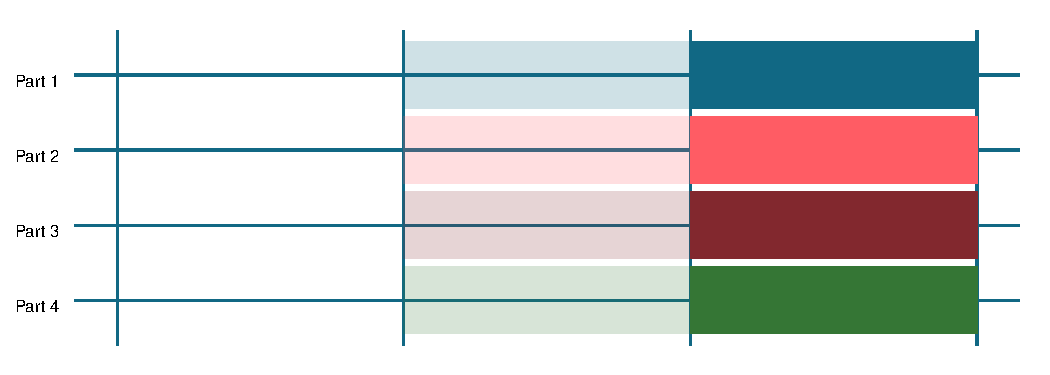
\includegraphics[width=\maxwidth,height=5cm]{figure/minimal-main-color} 

}



\end{knitrout}


These are the colors used mainly to generate the plots, and they are
chosen to be color blind proof. These colors can be obtained also from
the \textit{plot\_colors} function under the \textit{Sub} list where the
number of colors \textit{n} need to be specified.

\begin{knitrout}
\definecolor{shadecolor}{rgb}{0.969, 0.969, 0.969}\color{fgcolor}

{\centering 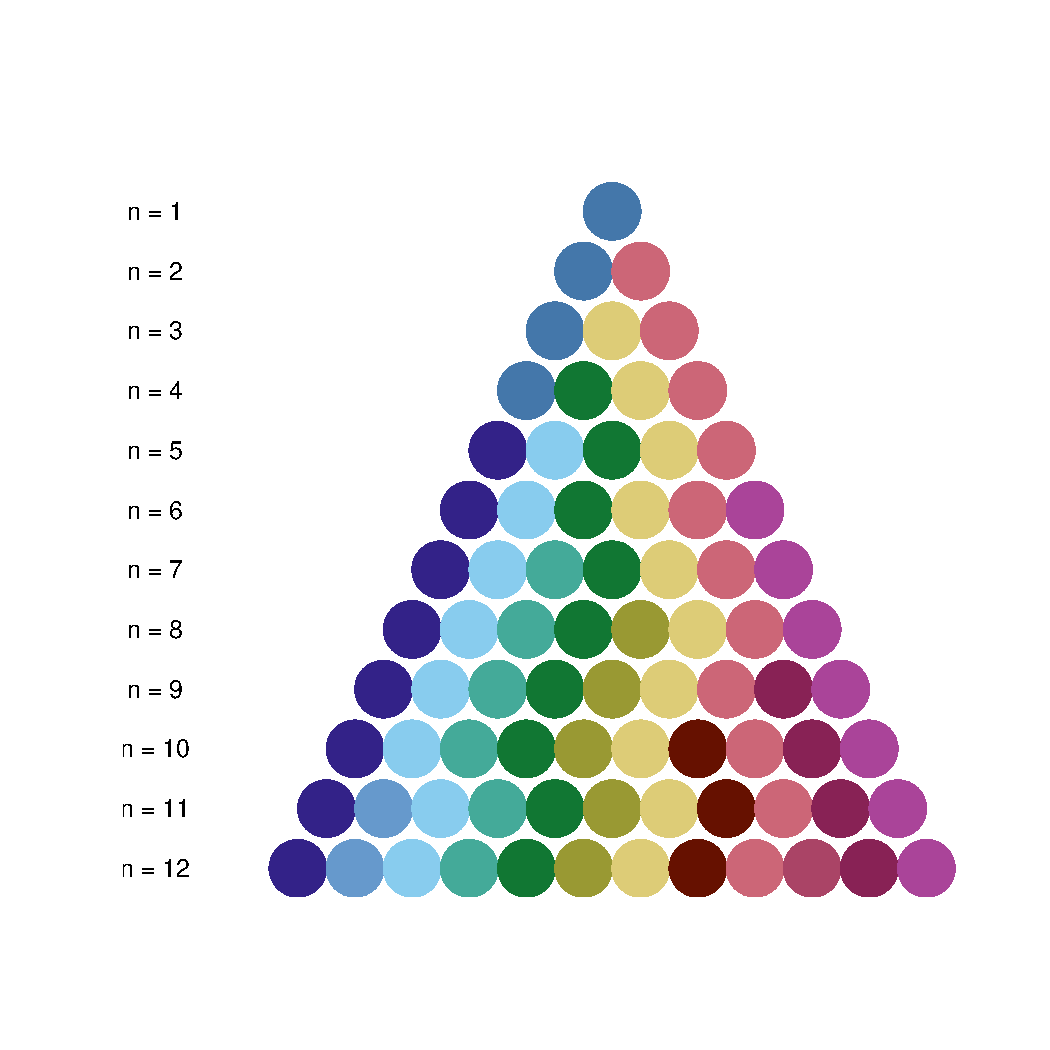
\includegraphics[width=\maxwidth]{figure/minimal-sub-color} 

}



\end{knitrout}



\section{Pre-defined plot}

\subsection{Single indicator}
The use of the graph is very simple, the four key components required
are the \textit{x}, \textit{y}, \textit{group} and the
\textit{type}. The x and y corresponds to the \textit{x} and
\textit{y} of \textbf{ggplot} and the \textit{group} factor determines
the color and finally the type is the pre-defined plot in the
\textit{plot\_dictionary}.


\subsubsection{Bar graph}
Now let us explore the data, the first graph available is the simple
bar chart. In this chart we have plotted the total population by
region, and it is clear that Asia has a much greater population and
Oceania has the smallest population.

\begin{knitrout}
\definecolor{shadecolor}{rgb}{0.969, 0.969, 0.969}\color{fgcolor}\begin{kframe}
\begin{alltt}
\hlfunctioncall{plot_syb}(x = \hlstring{"OFFICIAL_FAO_NAME"}, y = \hlstring{"SP.POP.TOTL"},
         subset = Year == 2005 & Area == \hlstring{"Region"},
         group = \hlstring{"OFFICIAL_FAO_NAME"}, type = \hlstring{"reg_uni_bar"}, data = all.df,
         col_pallete = \hlfunctioncall{plot_colors}(n = 5)$Sub)
\end{alltt}
\end{kframe}

{\centering 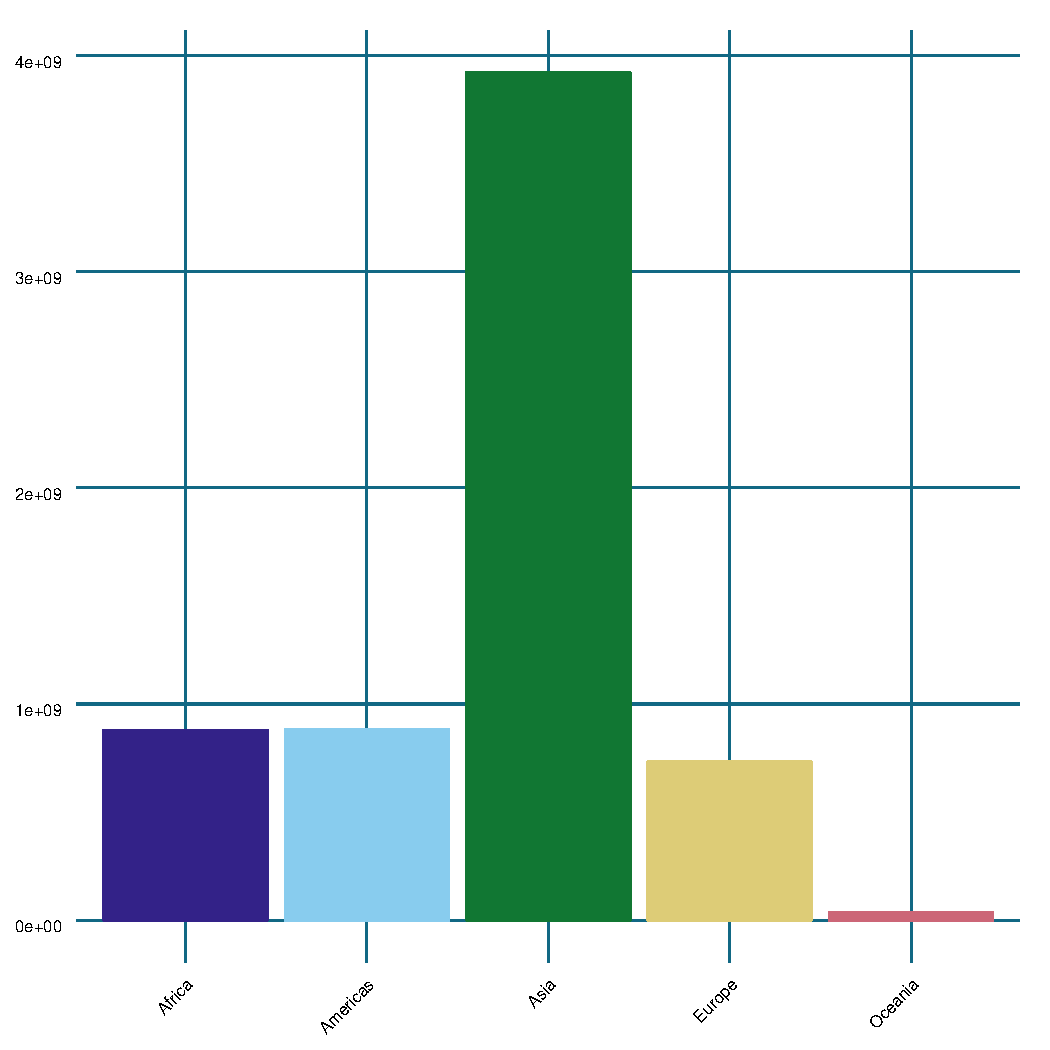
\includegraphics[width=\maxwidth]{figure/minimal-univariate-bar1} 

}



\end{knitrout}




\begin{knitrout}
\definecolor{shadecolor}{rgb}{0.969, 0.969, 0.969}\color{fgcolor}\begin{kframe}
\begin{alltt}
\hlfunctioncall{plot_syb}(x = \hlstring{"OFFICIAL_FAO_NAME"}, y = \hlstring{"SP.POP.TOTL"},
         group = \hlstring{"Year"}, type = \hlstring{"reg_uni_bar"},
         subset = Year %in% \hlfunctioncall{c}(1990, 2000, 2010) & Area == \hlstring{"Region"},
         data = all.df, col = \hlfunctioncall{plot_colors}(n = 3)$Sub,
         legend_lab = \hlfunctioncall{c}(1990, 2000, 2010))
\end{alltt}
\end{kframe}

{\centering 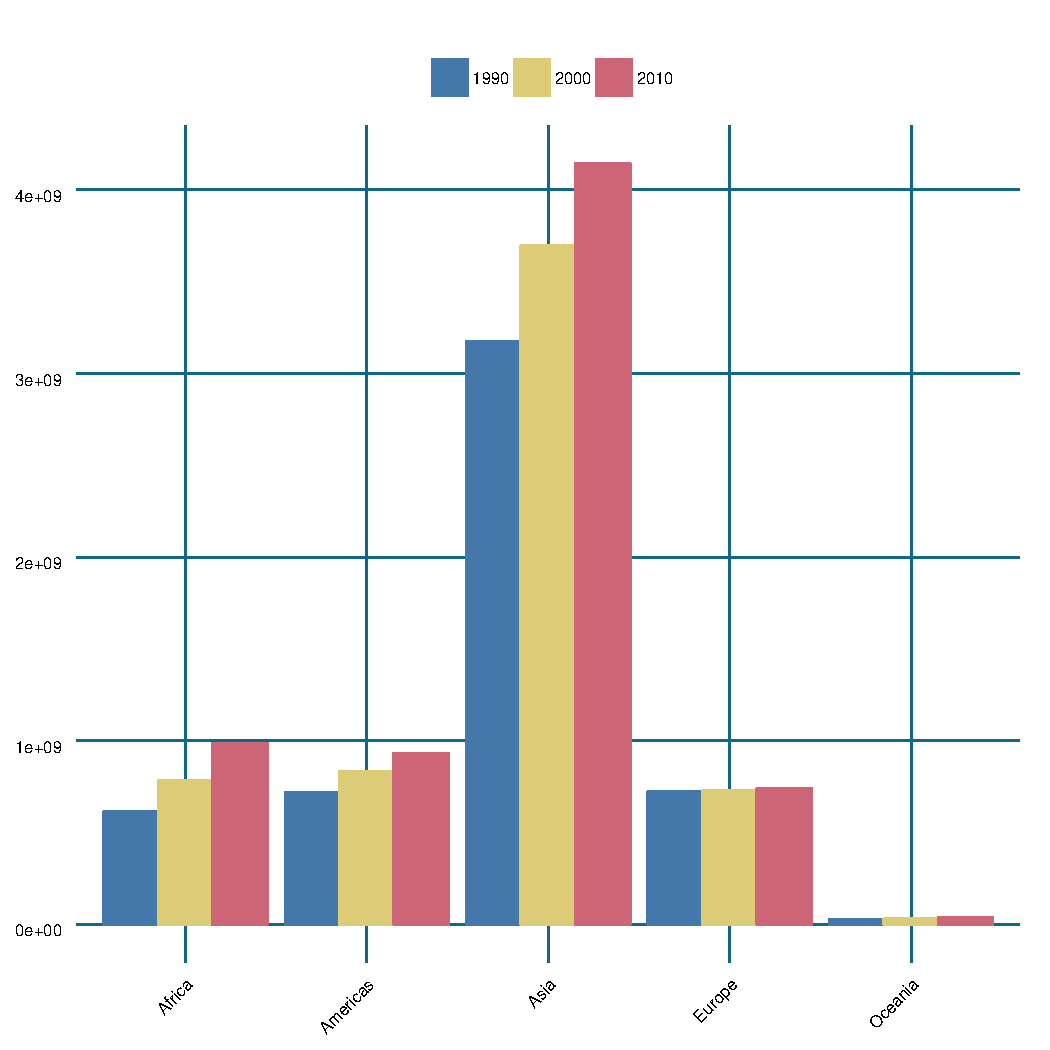
\includegraphics[width=\maxwidth]{figure/minimal-univariate-bar2} 

}



\end{knitrout}


This is a typical line graph.

\subsubsection{Line graph}
\begin{knitrout}
\definecolor{shadecolor}{rgb}{0.969, 0.969, 0.969}\color{fgcolor}\begin{kframe}
\begin{alltt}
\hlfunctioncall{plot_syb}(x = \hlstring{"Year"}, y = \hlstring{"SP.POP.TOTL"}, group = \hlstring{"OFFICIAL_FAO_NAME"},
         subset = Year %in% 1990:2010 & Area == \hlstring{"Region"},
         type = \hlstring{"reg_uni_line"}, data = all.df,
         col_pallete = \hlfunctioncall{plot_colors}(n = 5)$Sub)
\end{alltt}
\end{kframe}

{\centering 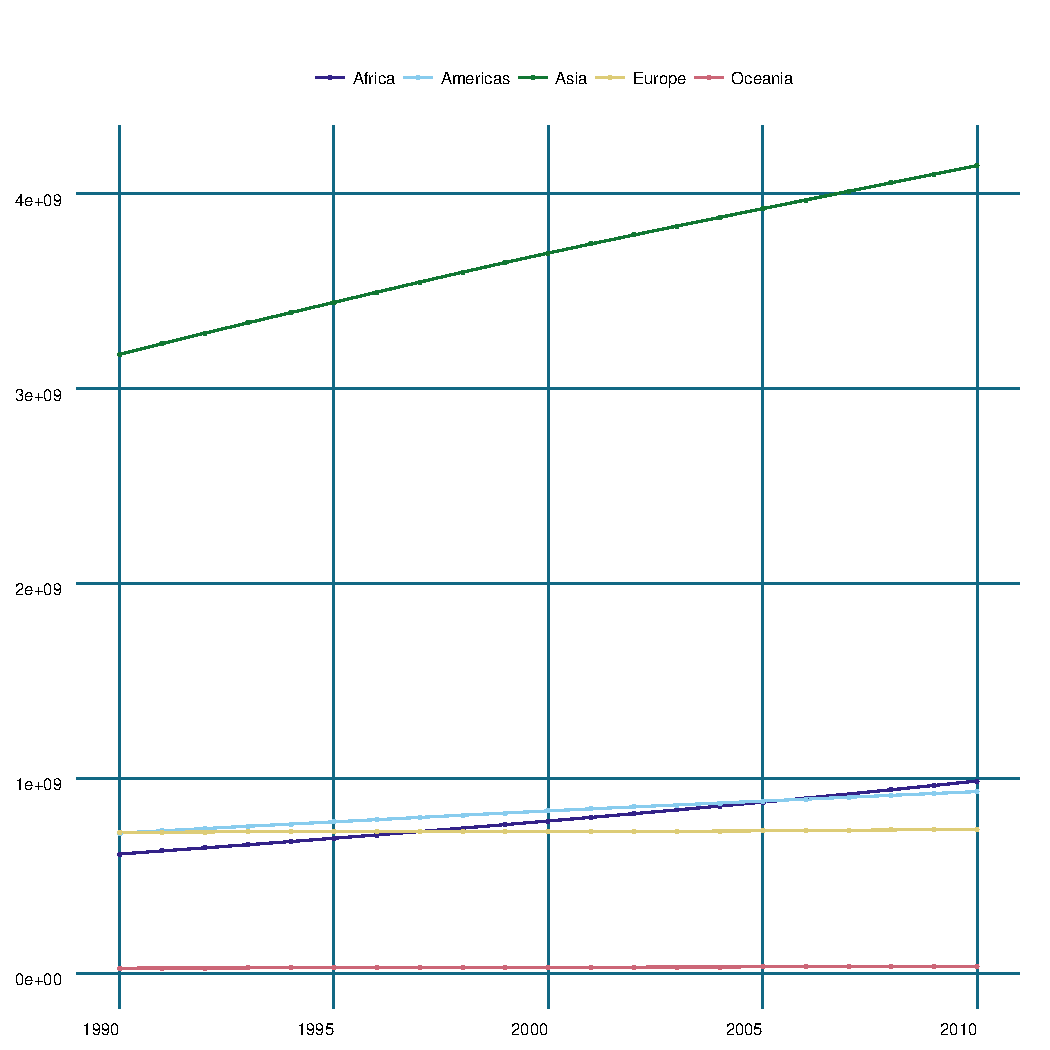
\includegraphics[width=\maxwidth]{figure/minimal-univariate-line} 

}



\end{knitrout}


\subsubsection{Top and bottom bar}
\begin{knitrout}
\definecolor{shadecolor}{rgb}{0.969, 0.969, 0.969}\color{fgcolor}\begin{kframe}
\begin{alltt}
\hlfunctioncall{plot_syb}(x = \hlstring{"SP.POP.TOTL"}, y = \hlstring{"OFFICIAL_FAO_NAME"},
         subset = Year ==  2010 & Area == \hlstring{"Territory"},
         type = \hlstring{"top_bot_bar"}, data = all.df,
         col_pallete = \hlfunctioncall{plot_colors}(n = 2)$Sub)
\end{alltt}
\end{kframe}

{\centering 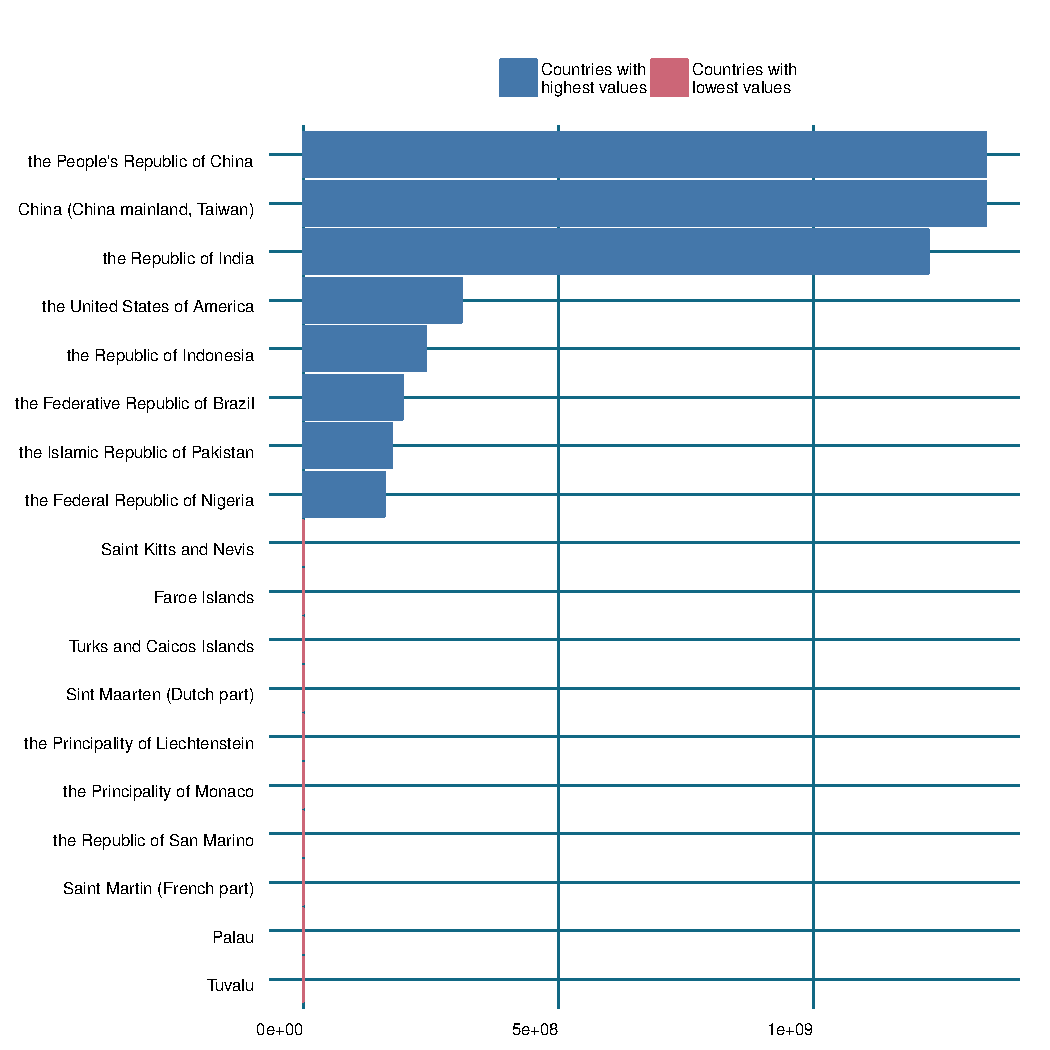
\includegraphics[width=\maxwidth]{figure/minimal-top-bot-bar} 

}



\end{knitrout}




\subsection{Multiple indicator}
Multiple indicators are supported, and the \textit{y} can be a
vector. The function will melt the data to form the standard
\textit{data.frame} used by \textbf{ggplot}.

\subsubsection{Scatter plot}

\begin{knitrout}
\definecolor{shadecolor}{rgb}{0.969, 0.969, 0.969}\color{fgcolor}\begin{kframe}
\begin{alltt}
\hlfunctioncall{plot_syb}(x = \hlstring{"SL.AGR.EMPL.MA.ZS"}, y = \hlstring{"NV.AGR.TOTL.ZS"},
         type = \hlstring{"scatter_plot"}, subset = Year == 2005 & Area == \hlstring{"Territory"},
         group = \hlstring{"UNSD_MACRO_REG"}, data = all.df,
         col_pallete = \hlfunctioncall{plot_colors}(n = 5)$Sub) +
    \hlfunctioncall{geom_smooth}(method = \hlstring{"lm"})

\end{alltt}
\end{kframe}

{\centering 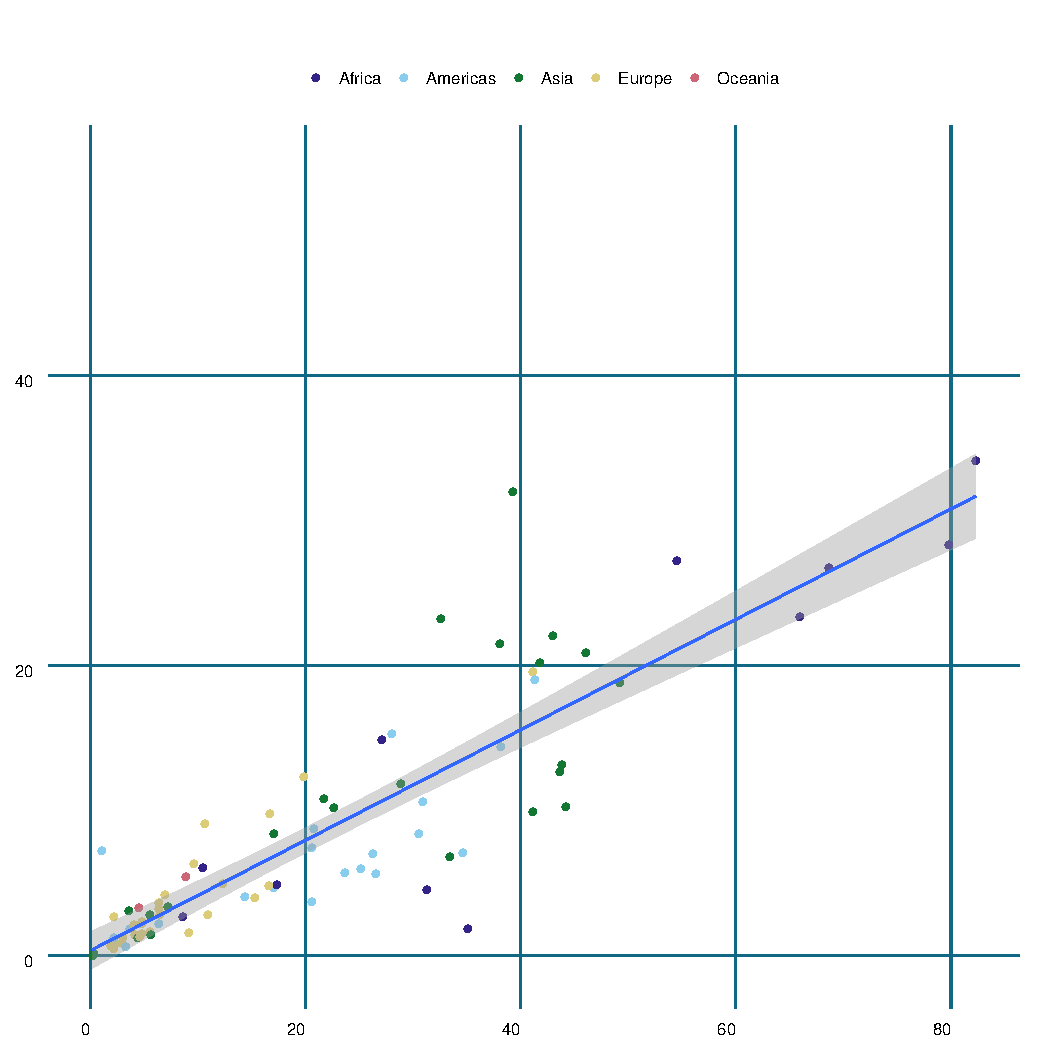
\includegraphics[width=\maxwidth]{figure/minimal-scatter-plot} 

}



\end{knitrout}





\subsubsection{Stacked bar graph}
\begin{knitrout}
\definecolor{shadecolor}{rgb}{0.969, 0.969, 0.969}\color{fgcolor}\begin{kframe}
\begin{alltt}
\hlfunctioncall{plot_syb}(x = \hlstring{"OFFICIAL_FAO_NAME"},
         y = \hlfunctioncall{c}(\hlstring{"SP.POP.0014.TO.ZS"}, \hlstring{"SP.POP.1564.TO.ZS"}, \hlstring{"SP.POP.65UP.TO.ZS"}),
         group = NULL, type = \hlstring{"multi_stack_bar"}, data = all.df,
         subset = Year == 2000 & Area == \hlstring{"Region"},
         col_pallete = \hlfunctioncall{plot_colors}(n = 3)$Sub,
         legend_lab = \hlfunctioncall{c}(\hlstring{"0 ~ 14"}, \hlstring{"15 ~ 64"}, \hlstring{"65+"}))
\end{alltt}
\end{kframe}

{\centering 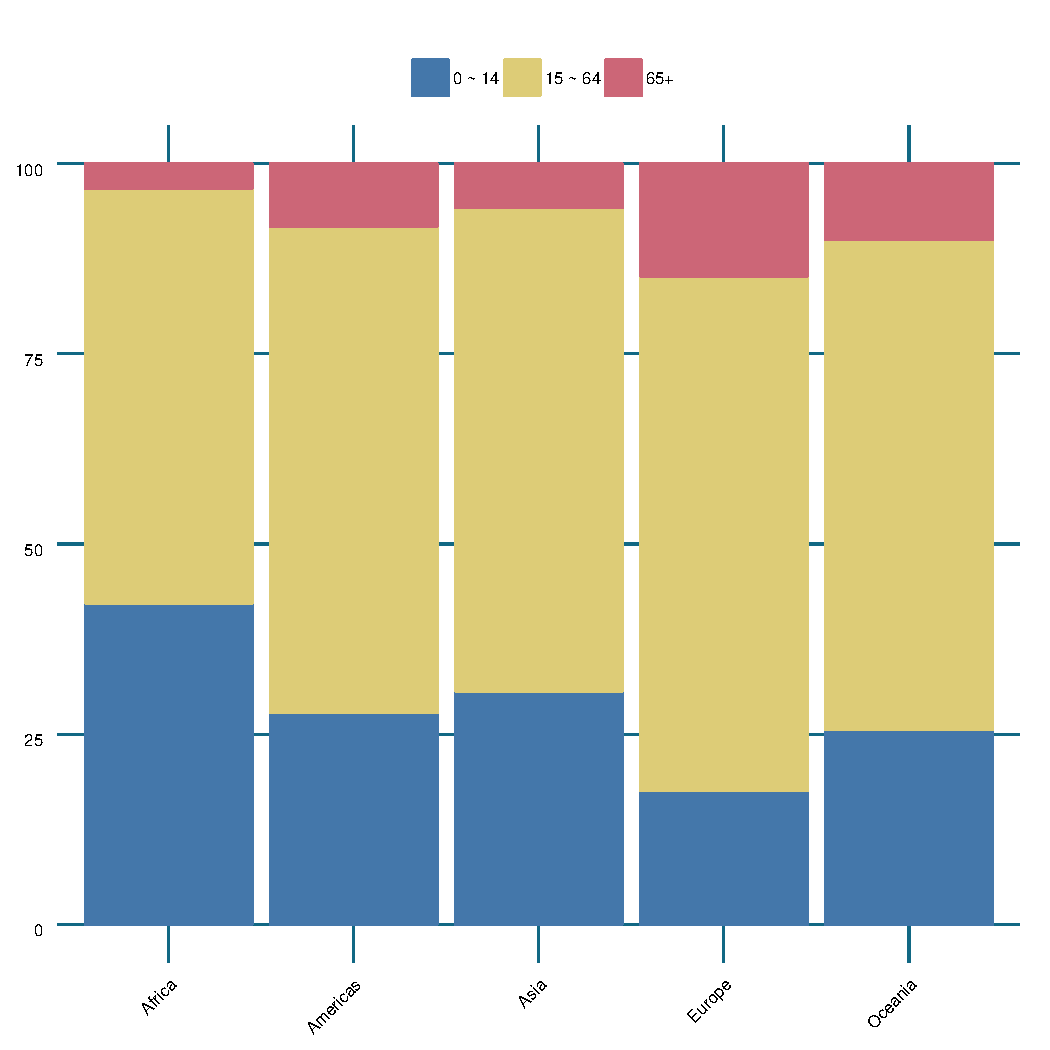
\includegraphics[width=\maxwidth]{figure/minimal-multivariate-stack-bar} 

}



\end{knitrout}


\subsubsection{Side-by-side bar graph}

\begin{knitrout}
\definecolor{shadecolor}{rgb}{0.969, 0.969, 0.969}\color{fgcolor}\begin{kframe}
\begin{alltt}
\hlfunctioncall{plot_syb}(x = \hlstring{"OFFICIAL_FAO_NAME"},
         y = \hlfunctioncall{c}(\hlstring{"SP.POP.0014.TO.ZS"}, \hlstring{"SP.POP.1564.TO.ZS"}, \hlstring{"SP.POP.65UP.TO.ZS"}),
         group = NULL, type = \hlstring{"multi_dodge_bar"}, data = all.df,
         subset = Year == 2000 & Area == \hlstring{"Region"},
         col_pallete = \hlfunctioncall{plot_colors}(n = 3)$Sub,
         legend_lab = \hlfunctioncall{c}(\hlstring{"0 ~ 14"}, \hlstring{"15 ~ 64"}, \hlstring{"65+"}))
\end{alltt}
\end{kframe}

{\centering 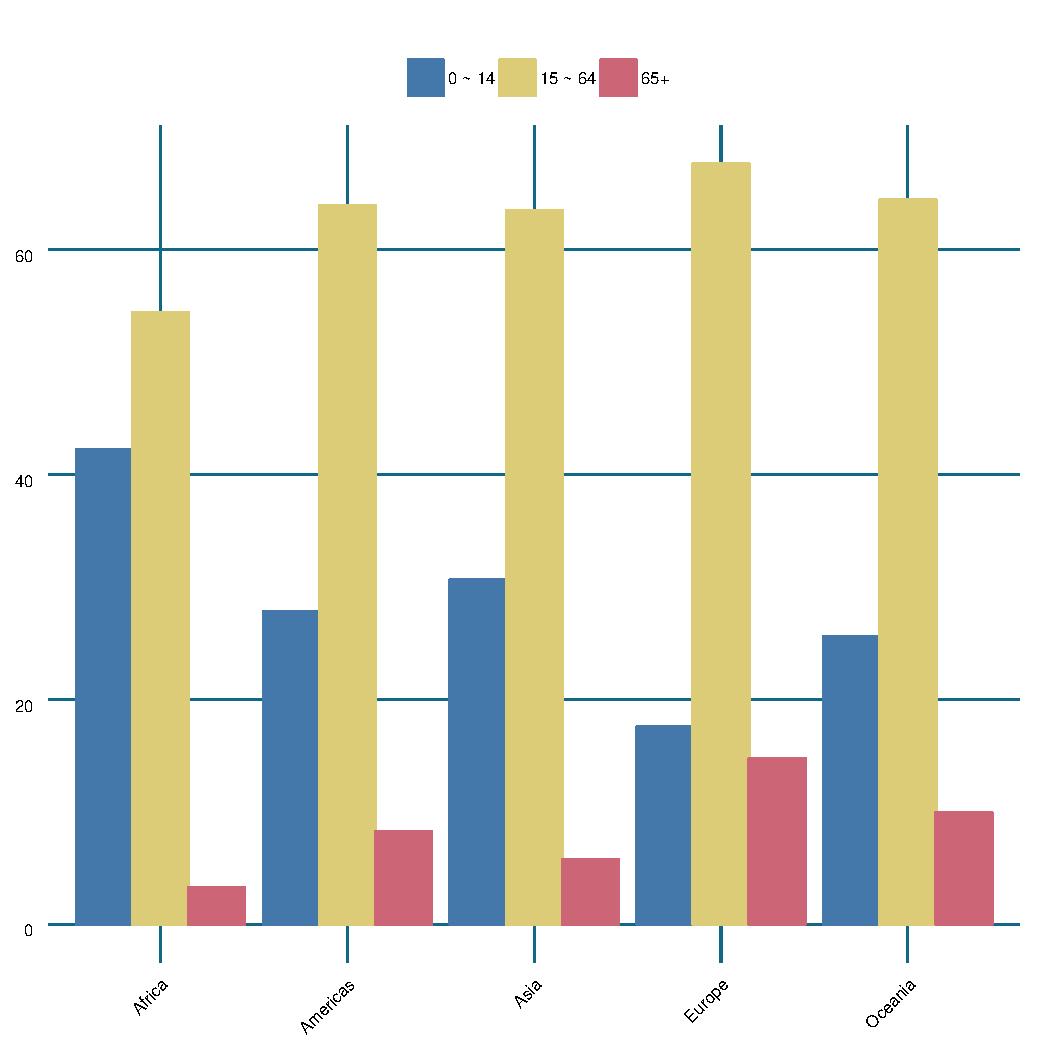
\includegraphics[width=\maxwidth]{figure/minimal-multivariate-dodge-bar} 

}



\end{knitrout}


\subsubsection{Area graph}
\begin{knitrout}
\definecolor{shadecolor}{rgb}{0.969, 0.969, 0.969}\color{fgcolor}\begin{kframe}
\begin{alltt}
\hlcomment{## Need to find a way to show the year points like the line graph}
\hlfunctioncall{plot_syb}(x = \hlstring{"Year"},
         y = \hlfunctioncall{c}(\hlstring{"SP.POP.0014.TO.ZS"}, \hlstring{"SP.POP.1564.TO.ZS"}, \hlstring{"SP.POP.65UP.TO.ZS"}),
         group = NULL, type = \hlstring{"multi_stack_line"},
         data = all.df, subset = Year %in% 2000:2010 &
             OFFICIAL_FAO_NAME == \hlstring{"Europe"},
         col_pallete = \hlfunctioncall{plot_colors}(n = 3)$Sub,
         legend_lab = \hlfunctioncall{c}(\hlstring{"0 ~ 14"}, \hlstring{"15 ~ 64"}, \hlstring{"65+"}))
\end{alltt}
\end{kframe}

{\centering 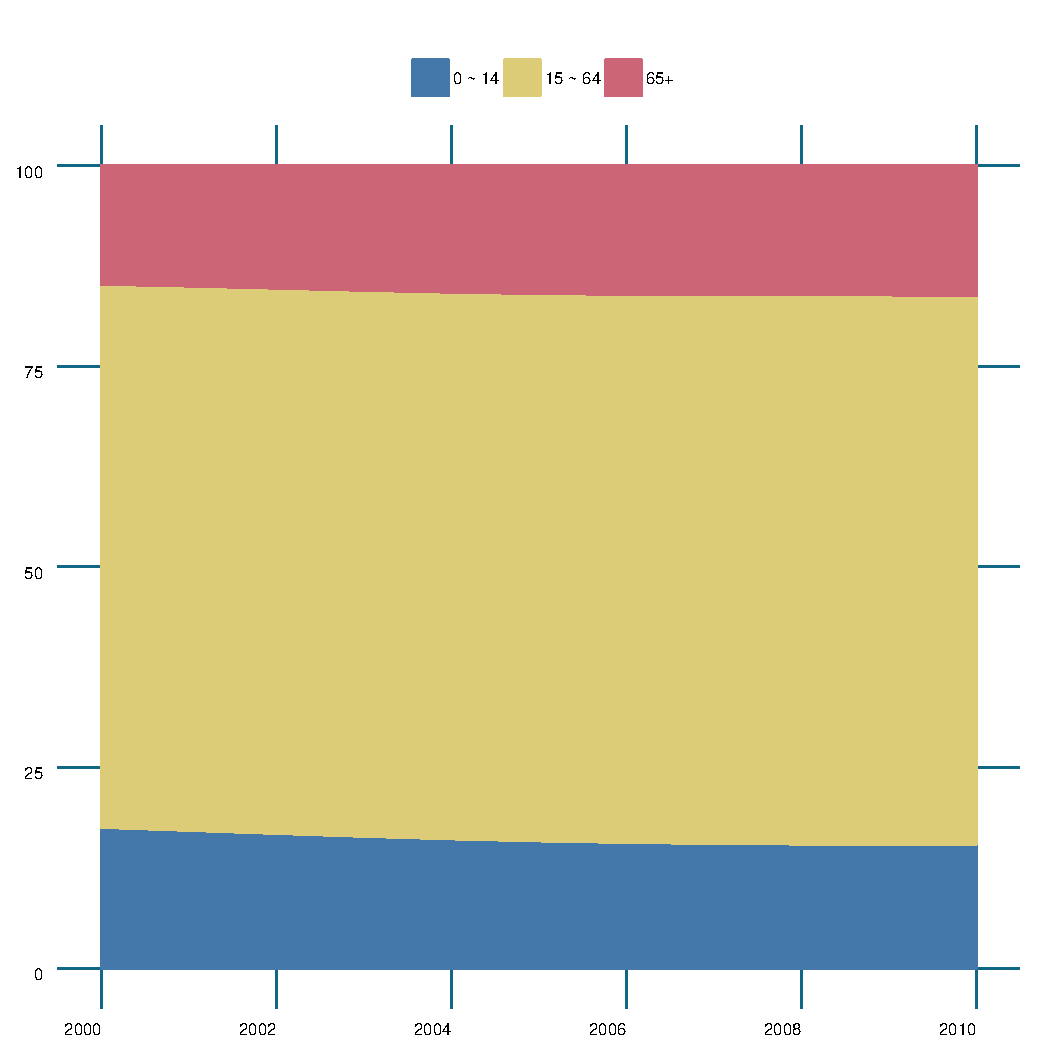
\includegraphics[width=\maxwidth]{figure/minimal-multivariate-stack-line} 

}



\end{knitrout}


\subsection{Maps}
\begin{knitrout}
\definecolor{shadecolor}{rgb}{0.969, 0.969, 0.969}\color{fgcolor}\begin{kframe}
\begin{alltt}
\hlfunctioncall{if}(!\hlfunctioncall{isTRUE}(\hlfunctioncall{gpclibPermitStatus}()))
    \hlfunctioncall{gpclibPermit}()
map.df = \hlfunctioncall{translateCountryCode}(data = all.df[all.df$Area == \hlstring{"Territory"}, ],
    from = \hlstring{"UN_CODE"}, to = \hlstring{"FAOST_CODE"})
\hlfunctioncall{plot_map}(var = \hlstring{"SP.POP.TOTL"}, data = map.df,
         countryCode = \hlstring{"FAOST_CODE"},
         subset = Year == 2010 & Area == \hlstring{"Territory"})
\end{alltt}
\end{kframe}

{\centering 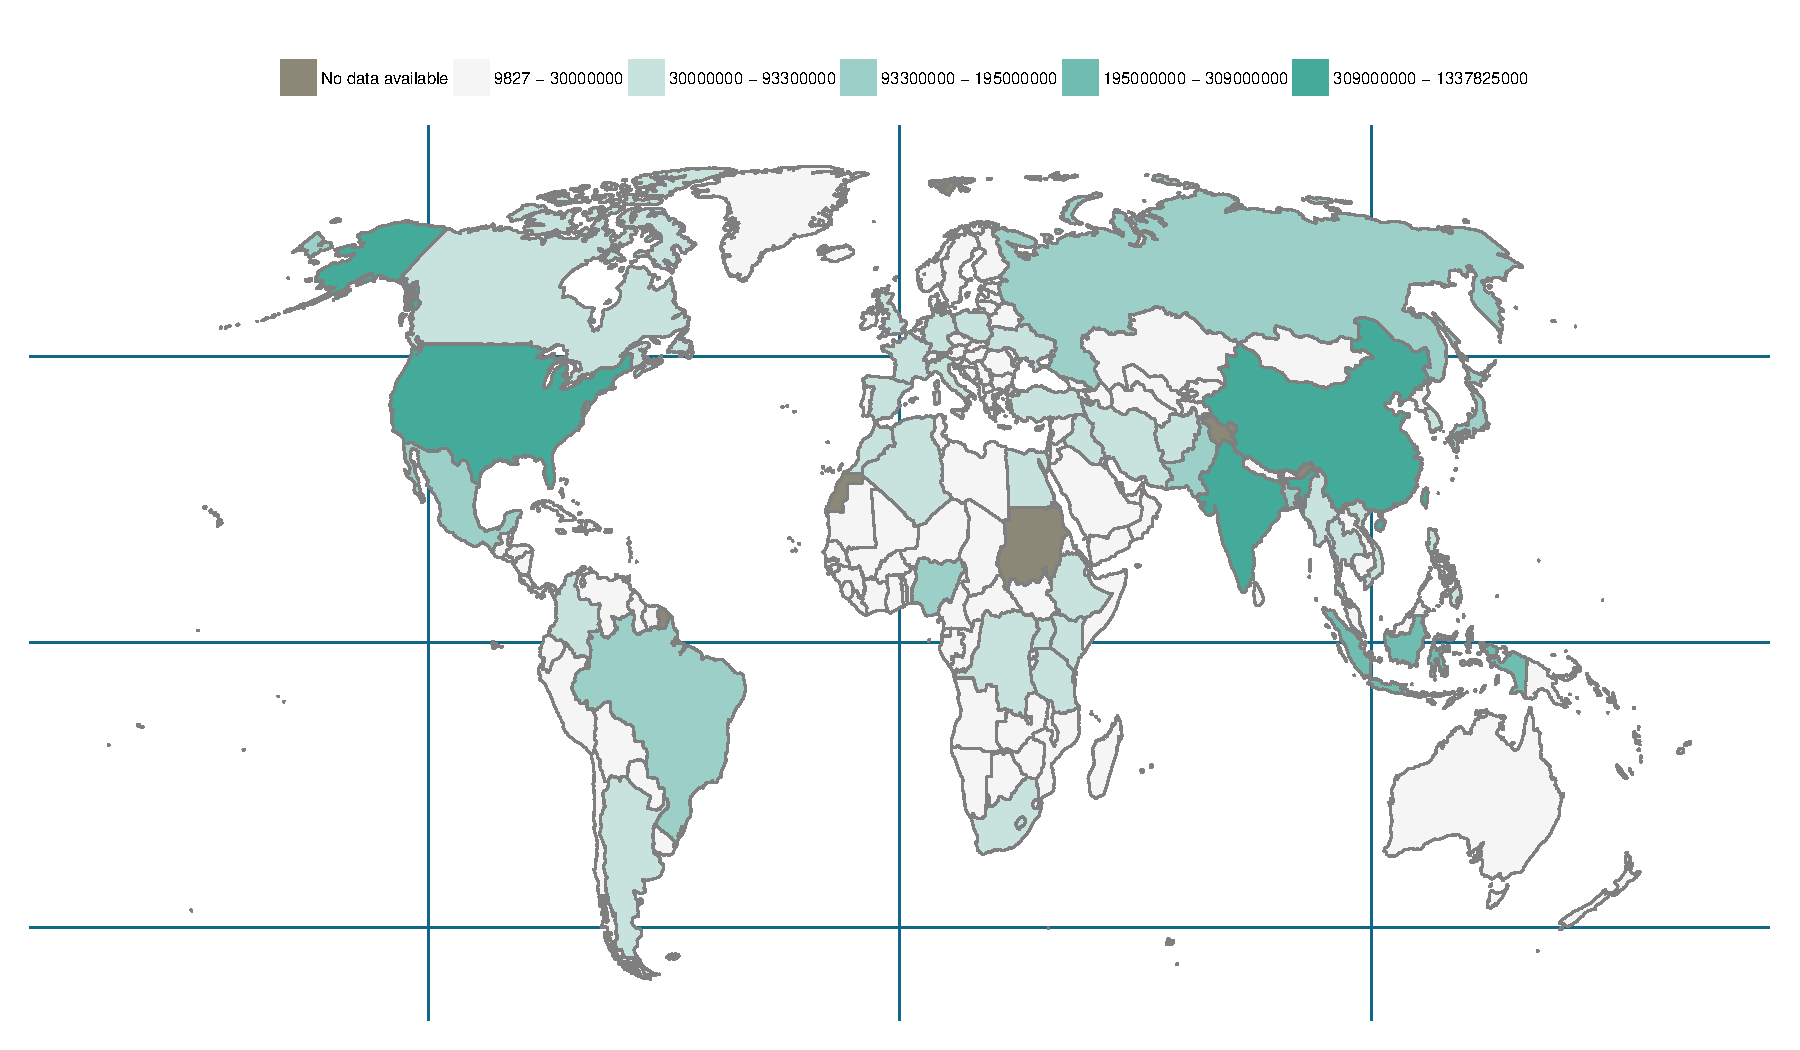
\includegraphics[width=\maxwidth]{figure/minimal-maps} 

}



\end{knitrout}


%% Need to wrap the European map



%% Need to find out why Sudan and some countries are missing



%% Need to fix the American map



%% Need to wrap the map



%% Asians are great!







\subsection{Diagnostic graph}
\begin{knitrout}
\definecolor{shadecolor}{rgb}{0.969, 0.969, 0.969}\color{fgcolor}\begin{kframe}
\begin{alltt}
\hlfunctioncall{dataDensity}(all.df[all.df$Year == 2008,
               \hlfunctioncall{colnames}(all.df)[!(\hlfunctioncall{colnames}(all.df) %in%
                                \hlfunctioncall{c}(\hlstring{"UN_CODE"}, \hlstring{"Year"}, \hlstring{"OFFICIAL_FAO_NAME"},
                                  \hlstring{"Area"}, \hlstring{"UNSD_MACRO_REGION"}))]]) +
    \hlfunctioncall{theme}(axis.text.x = \hlfunctioncall{element_blank}(),
          axis.ticks.x = \hlfunctioncall{element_blank}())
\end{alltt}


{\ttfamily\noindent\bfseries\color{errorcolor}{\#\# Error: object 'percent' not found}}\begin{alltt}

\end{alltt}
\end{kframe}
\end{knitrout}



%% implement subset for sparsityHeatMap
%% The following graph would only work on non-imputed data



\begin{knitrout}
\definecolor{shadecolor}{rgb}{0.969, 0.969, 0.969}\color{fgcolor}\begin{kframe}
\begin{alltt}
\hlfunctioncall{sparsityHeatMap}(data = all.df[all.df$Area == \hlstring{"Territory"}, ],
                country = \hlstring{"OFFICIAL_FAO_NAME"}, year = \hlstring{"Year"},
                var = \hlstring{"SP.POP.TOTL"}, group = \hlstring{"UNSD_MACRO_REG"})
\end{alltt}
\end{kframe}

{\centering 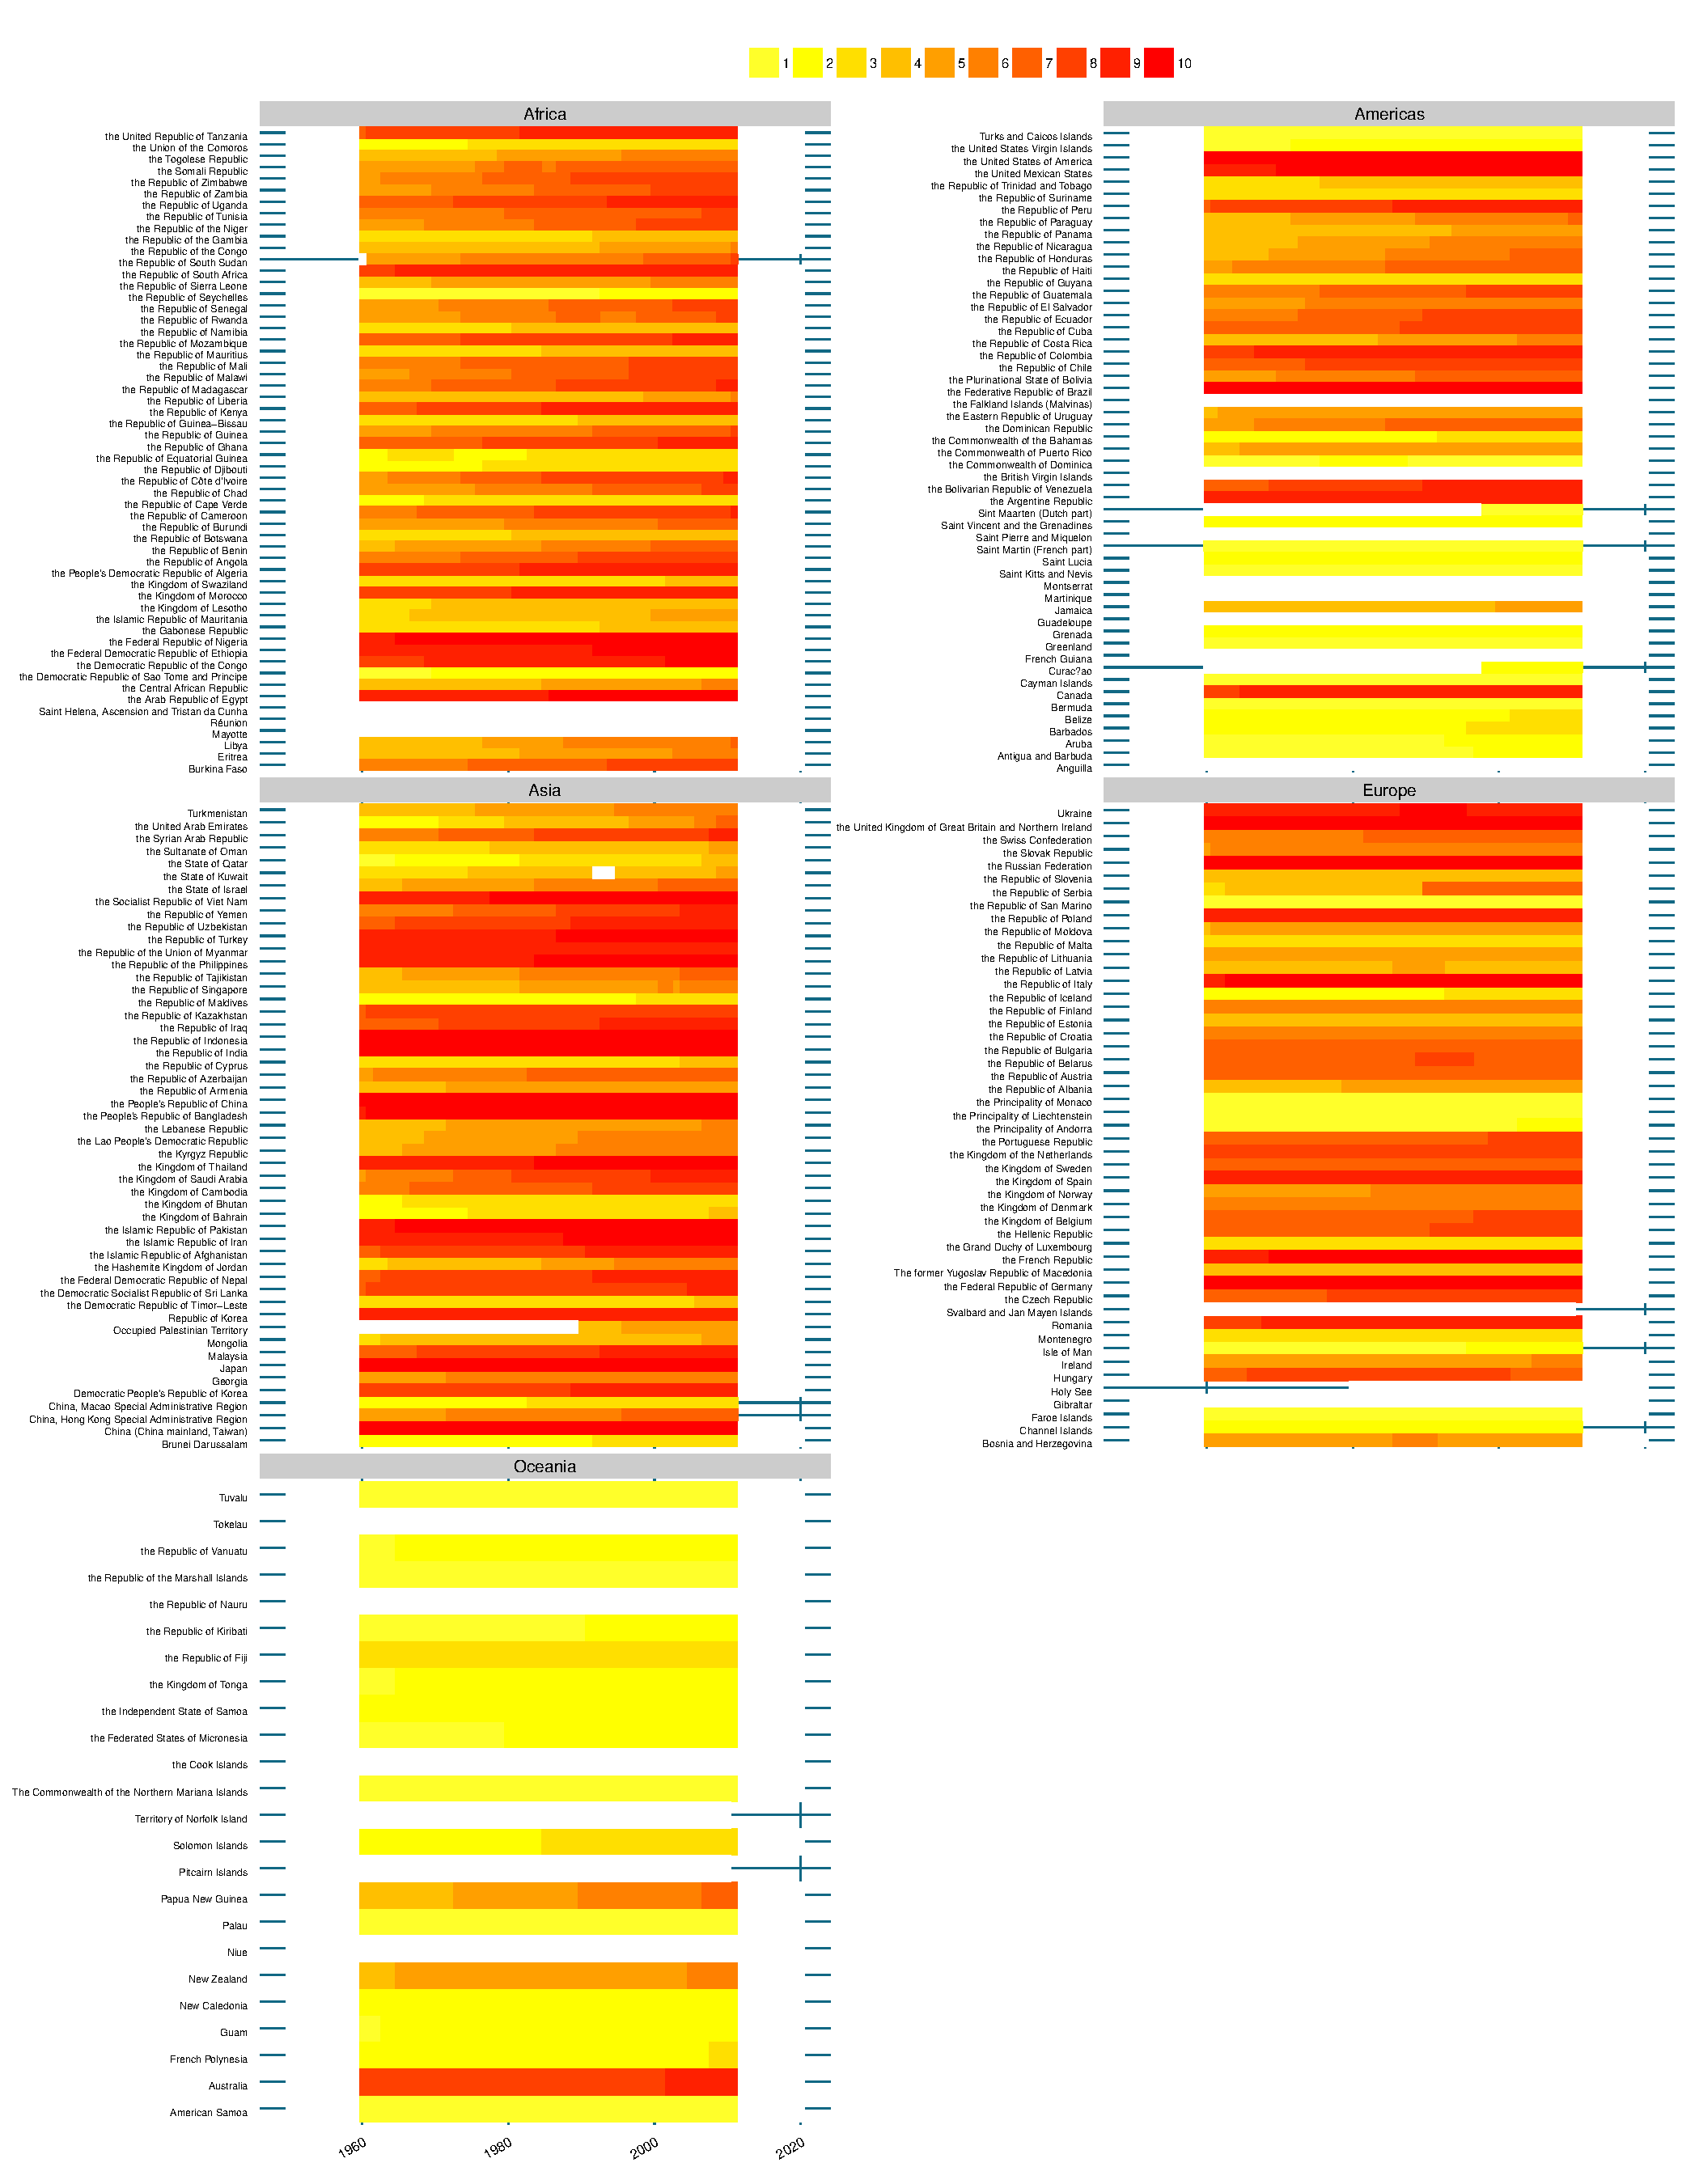
\includegraphics[width=\maxwidth]{figure/minimal-sparsity-heatmap2} 

}



\end{knitrout}









\end{document}
